\section{Particle-particle particle-mesh method}
The \PThreeM{} algorithm is a hybrid method:
forces between distant particles are calculated using the PM method, whereas for particles lying closely together the PP method is used.
The total force applied to particle $i$ is
\begin{equation}\label{eq:p3m}
    \mathbf{F}_i^\text{SR} + \mathbf{F}_i = \sum_{j \neq i}(\mathbf{f}_{ij}^\text{tot} - \mathbf{R}_{ij}) + \mathbf{F}_i,
\end{equation}
where $\mathbf{F}_i \approx \sum_{j\neq i} \mathbf{R}_{ij}$ is the force computed using the PM method and $\mathbf{R}_{ij} = \mathbf{R}(\mathbf{x}_i - \mathbf{x}_j)$ is a prescribed \textit{reference force}.
The reference force is defined as the force between two particle-clouds, i.e. each particle is represented by a sphere with diameter $a$ and a given density profile.
The two examples of reference forces described in \cite{Hockney1988} are
\begin{equation*}
    R(r) =
    G\times\begin{cases}
        \frac{1}{35  a^2}  (224  \xi - 224  \xi^3 + 70  \xi^4 + 48  \xi^5 - 21  \xi^6),                                & 0 \leq \xi \leq 1 \\
        \frac{1}{35  a^2}  (12 / \xi^2 - 224 + 896  \xi - 840  \xi^2 + 224  \xi^3 + 70  \xi^4 - 48  \xi^5 + 7  \xi^6), & 1 < \xi \leq 2    \\
        \frac{1}{r^2},                                                                                                 & \xi > 2
    \end{cases}
\end{equation*}
where $\xi = 2r/a$ for a sphere with uniformly decreasing density (shape $S_2$) and
\begin{equation*}
    R(r) =
    G\times\begin{cases}
        \frac{1}{a^2}  (8  r / a - 9  r^2 / a^2 + 2  r^4 / a^4), & r < a \\
        \frac{1}{r^2},
    \end{cases}
\end{equation*}
for a solid sphere (shape $S_1$).

\subsection{Optimal Green's function}
As it is apparent from \autoref{eq:p3m}, the method's validity depends on how well the reference force is approximated by the mesh force.
The average deviation between the two forces can be minimized by a suitable choice of the Green's function.
The details of the derivation are highly nontrivial and the can be found in \cite{Hockney1988};
in this work we restrict ourselves to presenting the results (essential to the implementation) obtained therein.

The optimal influence function $\hat{G}$ is given by
\begin{equation*}
    \hat{G}(\mathbf{k}) = \frac{\hat{\mathbf{D}}(\mathbf{k}) \cdot \sum_{\mathbf{n}}\hat{U}^2(\mathbf{k_\mathbf{n}}) \hat{\mathbf{R}}(\mathbf{k}_\mathbf{n})}{|\hat{\mathbf{D}}(\mathbf{k})|^2 \left[ \sum_{\mathbf{n}}\hat{U}^2(\mathbf{k}_\mathbf{n}) \right]^2}.
\end{equation*}
The Fourier transform $\hat{\mathbf{D}}$ of the two-point finite difference operator defined in \autoref{eq:two-point-central-diff} has the components
\begin{equation*}
    \hat{D}_j = \frac{i\sin k_j H}{H}
\end{equation*}
and for the four-point finite difference (\autoref{eq:four-point-central-diff}) we have
\begin{equation*}
    \hat{D}_j = \alpha\frac{i\sin k_j H}{H} + (1- \alpha)\frac{i\sin 2k_j H}{2H},
\end{equation*}
where $j=1,2,3$.
The quantity $\hat{U}$ is defined as $\hat{W}/V$.
For the mass assignment scheme hierarchy described in \autoref{subsec:mass-assignment} we have
\begin{equation*}
    \hat{U}(\mathbf{k}) = \left(\prod_{i=1}^{3}\frac{\sin(k_i H / 2)}{k_i H / 2}\right)^{p},
\end{equation*}
where $p=1,2,3,\dots$ with $p=1$ corresponding to NGP assignment, etc.
In particular, for the TSC assignment scheme, it can be shown that the \textit{alias sum}\footnote{
    To get the alias sums compatible with the DFT definition given in \autoref{eq:standard-dft}, one has to compute
    \begin{equation*}
        \sum_{\mathbf{n}} \tilde{U}^2(\mathbf{k}_\mathbf{n})
        \equiv \sum_\mathbf{n}\tilde{U}^2(\mathbf{k}+\mathbf{n}N)
        = \frac{1}{H}\sum_\mathbf{n}\hat{U}^2\left(\mathbf{k}\frac{2\pi}{NH}+\mathbf{n}\frac{2\pi}{H}\right)
    \end{equation*}
    instead.
}
\begin{equation*}
    \sum_{\mathbf{n}}\hat{U}^2(\mathbf{k}_\mathbf{n})
    \equiv \sum_{\mathbf{n}}\hat{U}^2\left(\mathbf{k} + \mathbf{n}\frac{2\pi}{H}\right)
\end{equation*}
evaluates to
\begin{equation*}
    \sum_{\mathbf{n}}\hat{U}_\text{TSC}^2(\mathbf{k}_\mathbf{n})
    = \prod_{i=1}^{3} \left(1 - \sin^2\frac{k_i H}{2} + \frac{2}{15}\sin^4\frac{k_i H}{2}\right).
\end{equation*}
This formula can be readily derived using the partial fractions expansion of the cotangent function \cite{aigner2018proofs},
\begin{equation*}
    \frac{(-1)^s}{s!}\frac{d^s}{dx^s}\cot x = \sum_{n=-\infty}^{\infty} \frac{1}{(x-n\pi)^{s+1}}.
\end{equation*}
Using the same approach, we can obtain similar results for the CIC and NGP schemes, namely
\begin{equation*}
    \sum_{\mathbf{n}}\hat{U}_\text{CIC}^2 = \frac{1}{3} \prod_{i=1}^{3}  \left(1 + 2\cos^2\frac{k_i H}{2}\right)
    \quad \text{and} \quad
    \sum_{\mathbf{n}}\hat{U}_\text{NGP}^2 = 1.
\end{equation*}
The quantity $\hat{\mathbf{R}}$, the transformed reference force, is related to the shape $S$ of the particle-cloud by
\begin{equation*}
    \hat{\mathbf{R}}(\mathbf{k}) = -\frac{i\mathbf{k}\hat{S}^2(k)}{k^2},
\end{equation*}
where $k = |\mathbf{k}|$.
For spherically symmetric shapes $S$ we have
\begin{equation*}
    \hat{S}(k) = 4\pi \int_{0}^{\infty} r^2 S(r)\frac{\sin kr}{kr}dr.
\end{equation*}
This integral, evaluated for the $S_1$ and $S_2$ shapes respectively, gives
\begin{equation*}
    \hat{S_1}(k) = \frac{3}{(ka/2)^3}  \left(\sin\frac{ka}{2} - \frac{ka}{2} \cos\frac{ka}{2}\right)
\end{equation*}
and
\begin{equation*}
    \hat{S_2}(k) = \frac{12}{(ka/2)^4}\left(2 - 2\cos\frac{ka}{2}-\frac{ka}{2}\sin\frac{ka}{2}\right).
\end{equation*}
The infinite sum in the numerator does not have a closed form but this does not pose a problem since the summand decays rapidly with $\mathbf{n}$ moving further away from zero.

The result of applying the optimal Green's function in \autoref{eq:poisson-fourier-product} is shown in \autoref{fig:reference-force-approx}.
\begin{figure}[htp]
    \centering
    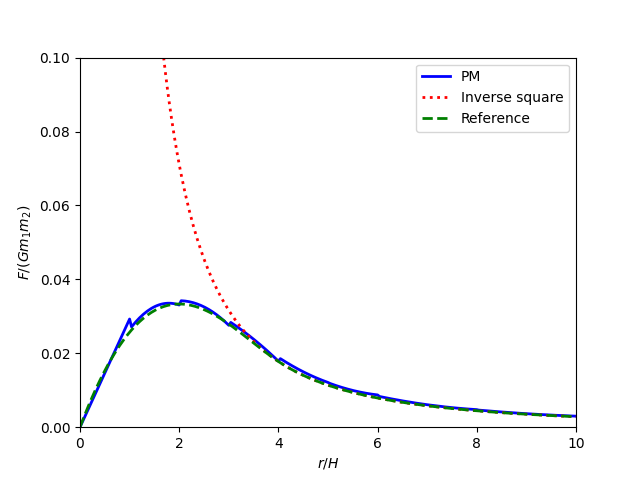
\includegraphics[scale=0.6]{img/optimal-green-force-4.png}
    \caption{Magnitude of the force between two masses.
        The mesh approximation to the reference force was calculated using the PM method with TSC assignment scheme, two-point finite difference, and the Green's function optimal for the $S_1$ shape with diameter $a=4H$.
        The force resultant from the universal law of gravitation is also shown.}
    \label{fig:reference-force-approx}
\end{figure}
As can be seen in the figure, the PM force closely follows the reference force.
Moreover, for $r>a$, the reference force is identical to the inverse-square force.
It is also worth noting that the reference force (and its mesh approximation) approximate the inverse-square force accurately for $r$ slightly smaller than $a$.
For this reason $r_e$, the \textit{cutoff radius} designating the boundary of the region handled by the direct summation, can be chosen to be smaller than $a$ (e.g. $r_e = 0.7a$).
This can have noticeable positive impact on performance.

\subsection{Identifying close pairs of particles}
